\section{Results and Discussion}\label{sec:result}

\comments{
{\color{red}{SS: Any need to list the number of steps we take to generate final model?}}

The step of shape optimization in our paper can be best demonstrated on the model Figure~\ref{fig:result}, through initialization, we can have a rough concept of the final model, and by user interaction including selecting vertexes merged and faces in the same plane, we can finally generate a pleasing model from a given structural layout.
}


Based on the two-step approach of folding a carton model as well as the suggestive user interface, our system is natural and easy to use. 
%
We will discuss a series of results to demonstrate the efficiency of our method. 


For most cuboid cartons, their 3D models can be generated by folding each edge by $\pi/2$, as shown Figure~\ref{fig:initial-automatic} and Figure~\ref{fig:automatic-more}.
In the common design process nowadays, designers typically spend much time on manually creating the 3D carton models in 3D modeling softwares. 
Our suggestive modeling interface saves the designers' effort significantly so that they could focus on carton appearance designing. 


\begin{figure}
	\centering
	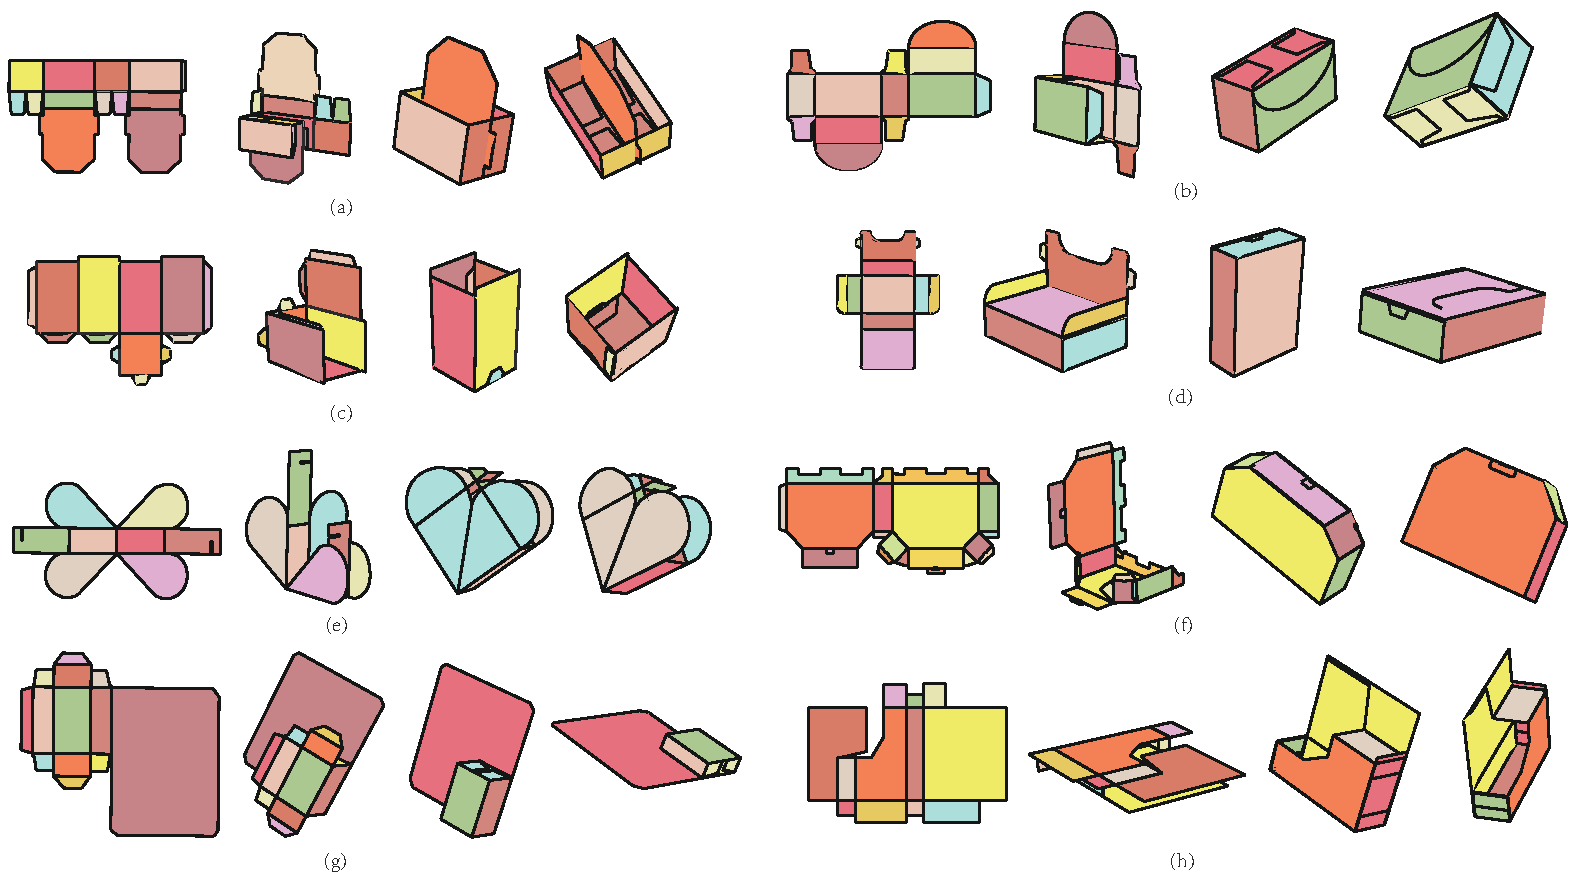
\includegraphics[width=\textwidth]{images/moreAutomatic}
	\caption{More carton examples that can be automatically generated.}
	\label{fig:automatic-more}
	
\end{figure}


If shape refinement is required, the entire process of creating a carton model from a 2D layout is illustrated in Figure~\ref{fig:result}.
The final model can be generated by three clicks for the user to confirm vertex merging two times, and face pasting in one time. 

\begin{figure}
	\centering
	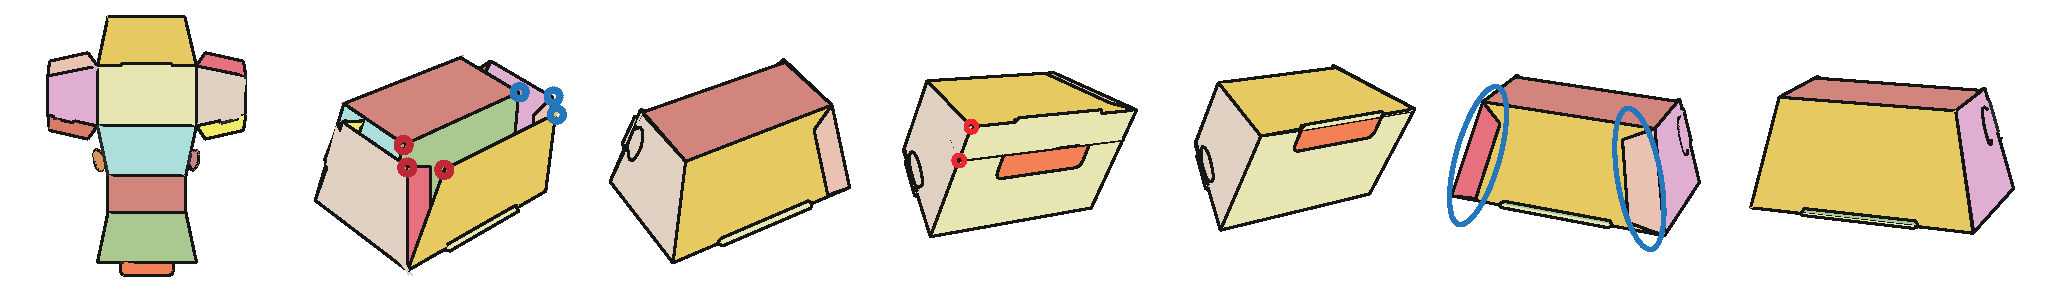
\includegraphics[width=\textwidth]{images/105}
	\caption{Structural layout is used to generate flat polymesh, and then initialize to a rough model, after two vertex merging confirmations and one face pasting confirmation, we can finally have its corresponding 3D model.}
	\label{fig:result}
\end{figure}
%
A more challenging example is shown in Figure~\ref{fig:hexagon}. 
By initially folding each edge as $\pi/2$, our system firstly generates a cube inside the carton for the six square faces. 
At the mean time, our system fails to detect mergeable vertexes with a small threshold $\epsilon$ to merge closeby vertexes.
%
However, the user could manually select two vertexes to merge. Then our systems automatically detects two symmetric vertexes that also can be merged. 
%
Finally, a hexagonal carton can be generated in a limited number of user interactions.

\comments{
However, the initialization will not generate a pleasing result on some complicated cases, and leads to the difficult interaction to get the final model. As for Figure~\ref{fig:hexagon}, to have a better corresponding model, users need to take at least ten steps to get to Figure~\ref{fig:hexagon}(c). 
}


\begin{figure}
	\centering
	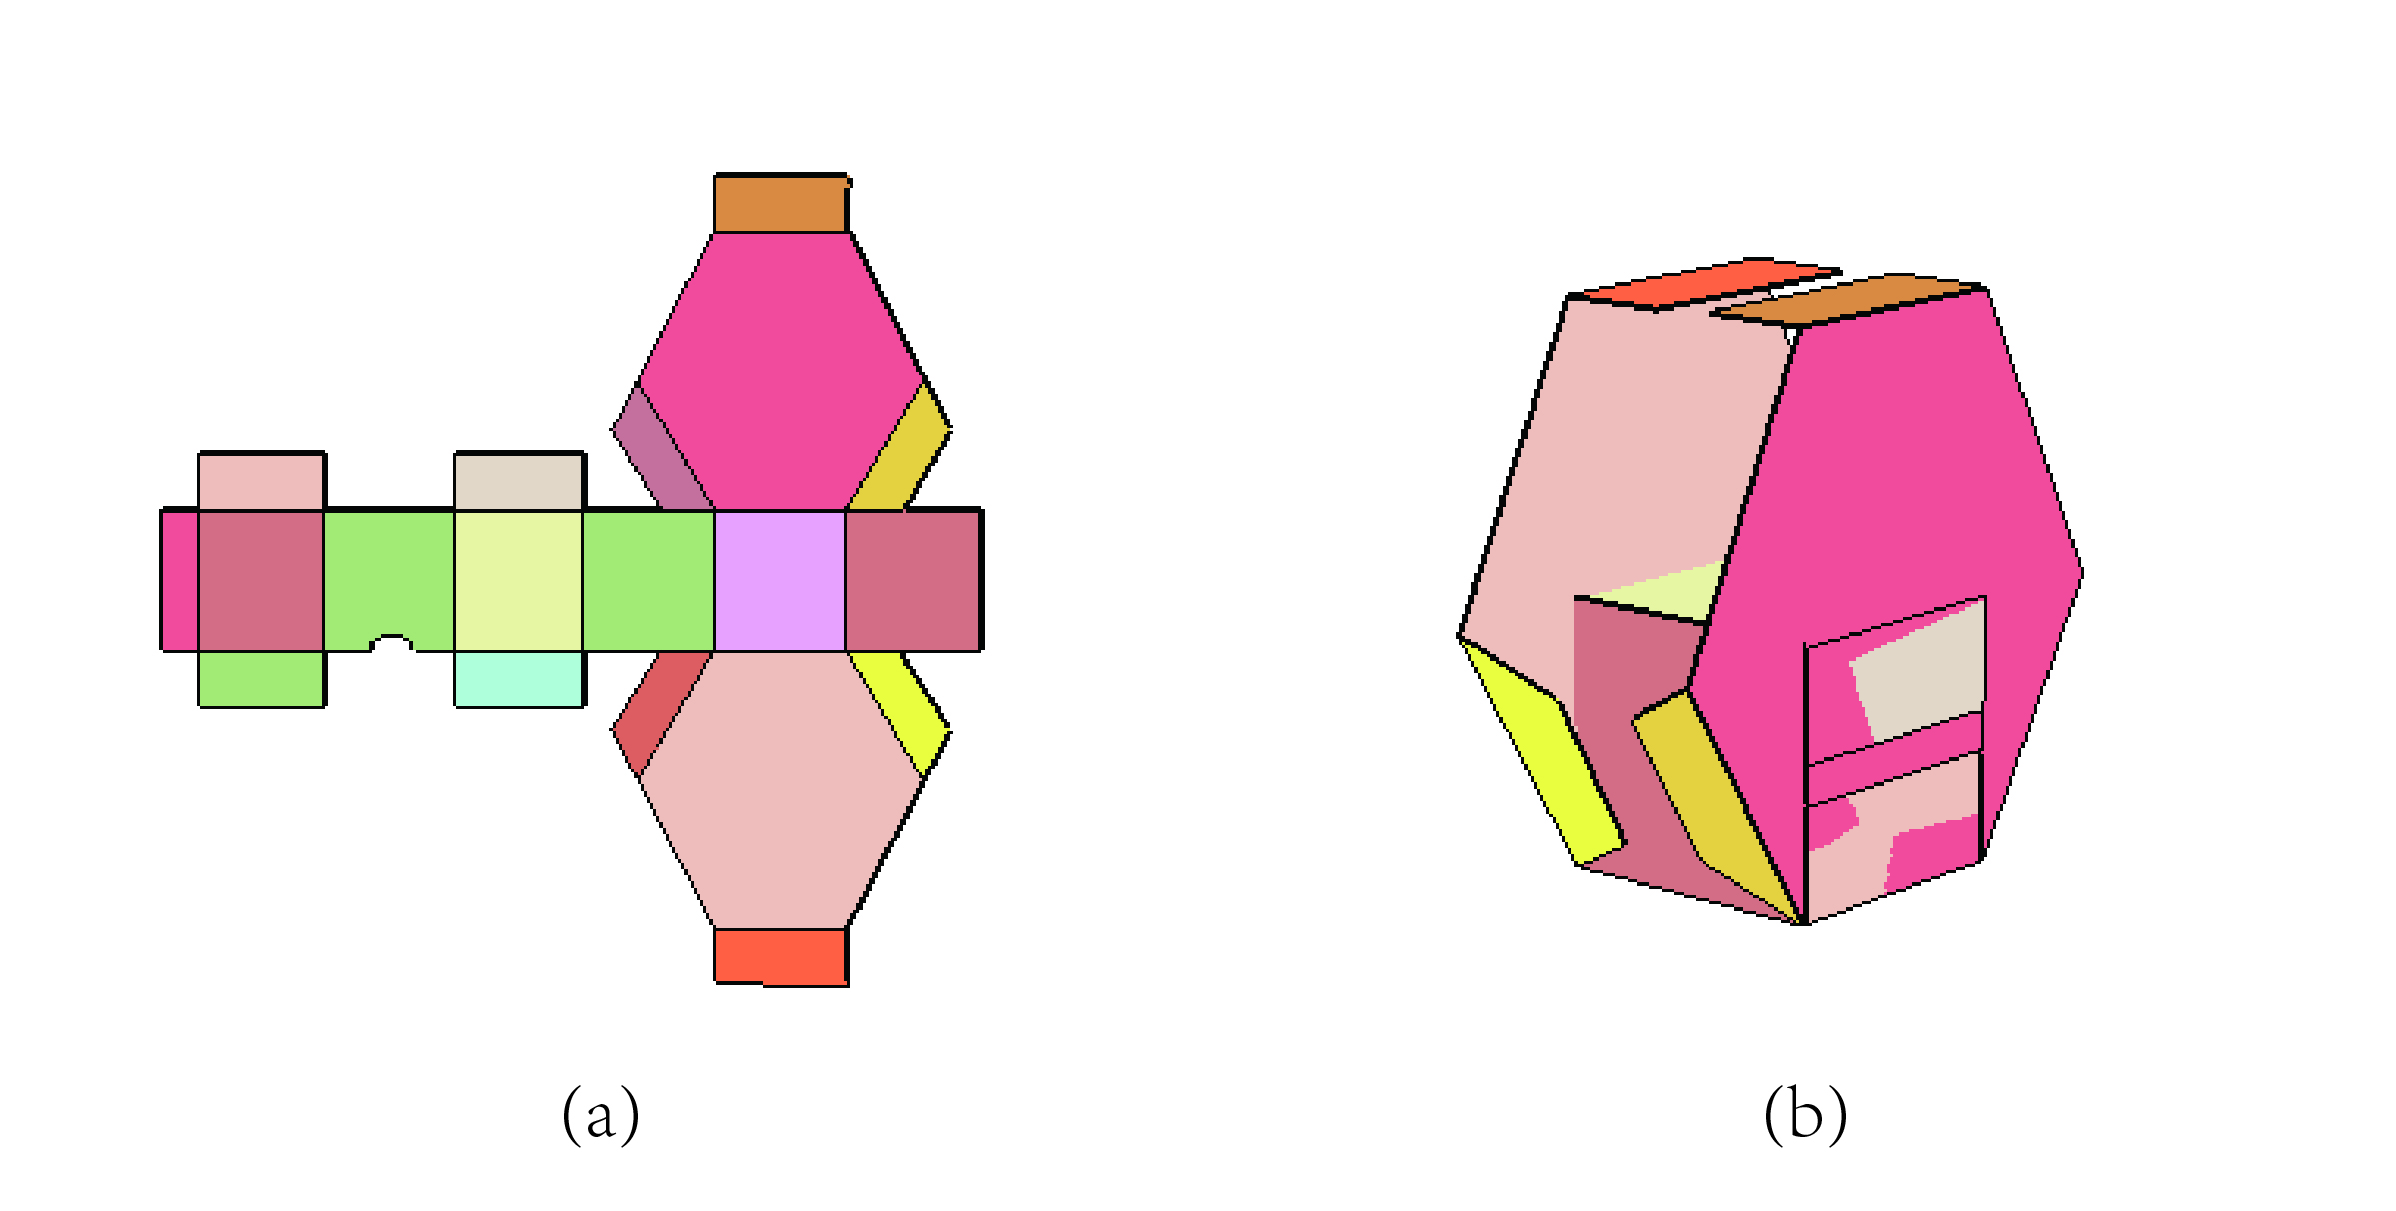
\includegraphics[width=0.9\textwidth]{images/limitation}
	\caption{Given a layout as (a), our system can generate an initialized result as (b), and through almost ten steps including selecting merging vertexes and faces need to be coplane , users can reach the final model as (d). }
	\label{fig:hexagon}
\end{figure}

\reply{
Shape optimization can be used in most cases through interaction, however, there are still some failure cases that we can not deal with. Figure~\ref{fig:failure} shows a case that failed to generate 3D model by optimization. The faces circled in red should be merged together to produce a strong enforced face, while our system expanded the face away. Moreover, we cannot deal with the case that if we want to layout down the back red face and keep the bottom lines of green side faces together. The carton layouts whose face graph has a loop will also be failed to construct corresponding model such as milk cartons.  
}

\begin{figure}
	\centering
	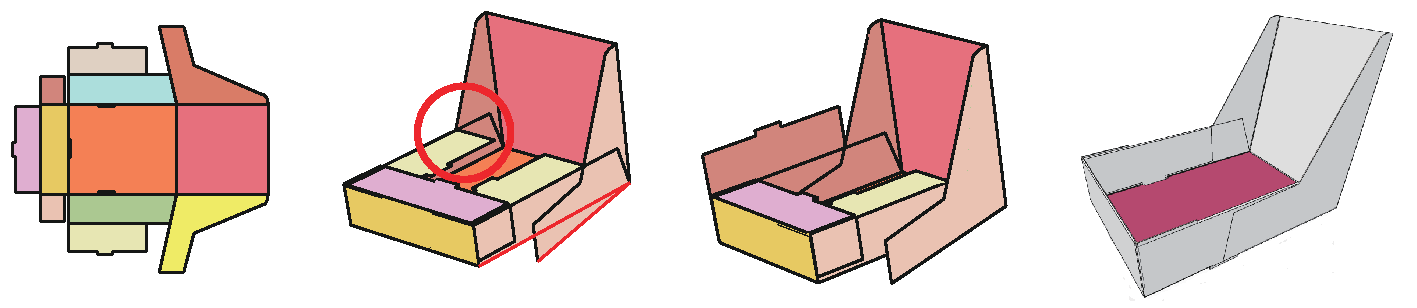
\includegraphics[width=0.9\textwidth]{images/moreLimitation}
	\caption{A failure case that shape optimization can not handle with. }
	\label{fig:failure}
\end{figure}

More carton models generated using our system are shown in Figure~\ref{fig:result-more}.
%and most of the cases can have an ideal result after initialization because of the cuboid shape as Figure~\ref{fig:more} (a). 
%
The statistics of the face number, edge number, and number of user interactions are listed in Table~\ref{table:statistics}. 
We can see that only a few user interactions on confirming system suggestions are needed for a variety of shapes.


\begin{table}
	\centering
	\caption{Statistics on the number of edges $N_{edge}$, number of faces $N_{face}$, and the number of user interactions $N_{interaction}$ of the examples shown in this paper.}
	\setlength{\tabcolsep}{1pt}
	\begin{tabular}{c|c|c|c|c|c|c|c|c|c|c|c|c}
		\hline
		Examples & Fig.\ref{fig:automatic-more}(a) & Fig.\ref{fig:automatic-more}(b) &  Fig.\ref{fig:automatic-more}(c) & Fig.\ref{fig:automatic-more}(d) & Fig.\ref{fig:result} & Fig.\ref{fig:hexagon} & Fig.\ref{fig:result-more}(a) & Fig.\ref{fig:result-more}(b)& Fig.\ref{fig:result-more}(c) &  Fig.\ref{fig:result-more}(d) & Fig.\ref{fig:result-more}(e)& Fig.\ref{fig:result-more}(f)\\
		\hline
		$N_{edge}$ & 49 & 62 & 46 & 45 & 54 & 67 & 40 & 43 & 42 & 38 & 48 & 30\\
		$N_{face}$  & 13 & 13 & 11 & 13 & 14 & 19 & 11 & 13 & 13 & 13 & 12 & 11\\
		$N_{interaction}$  & 0 & 0 & 0 & 0 & 3 & 9 & 1 & 4 & 1 & 3 & 3 & 3\\ 
		\hline
		\end{tabular}
		\label{table:statistics}
\end{table}



\begin{figure}
	\centering
	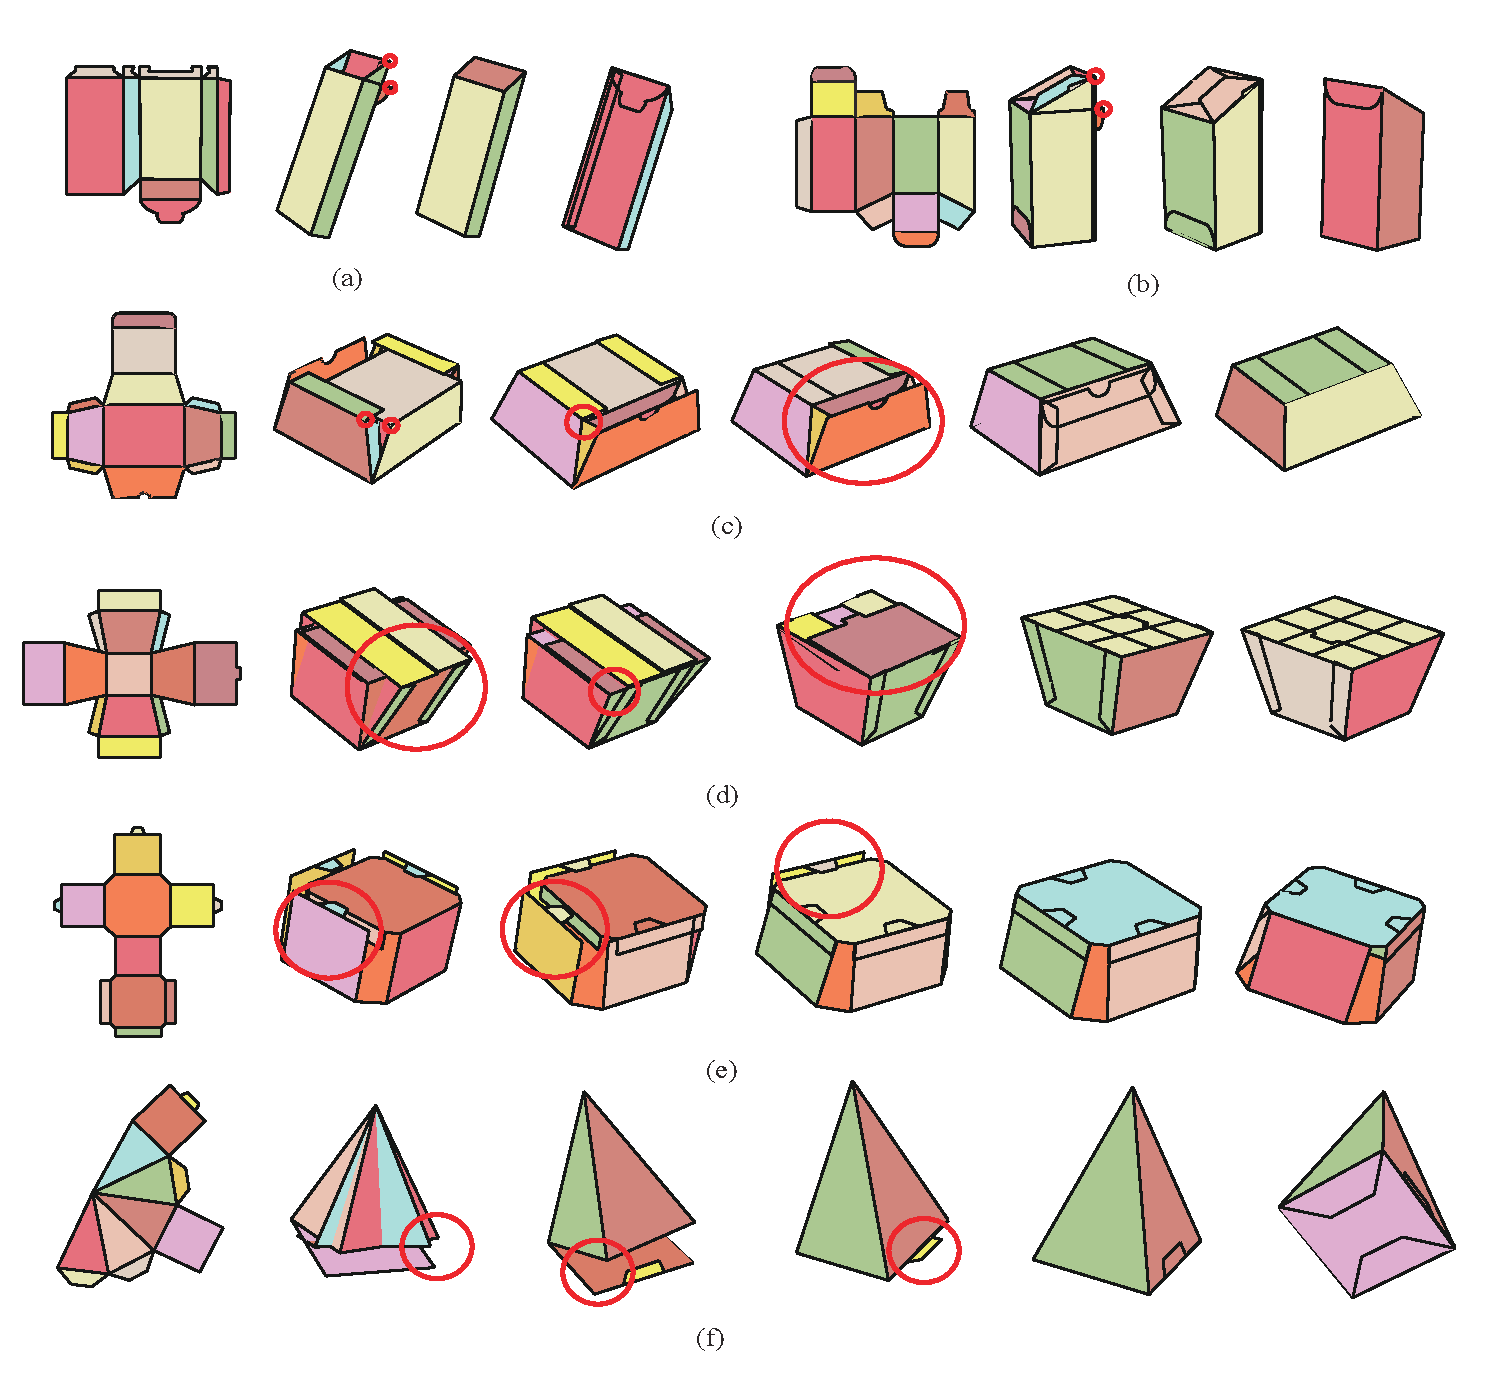
\includegraphics[width=0.9\textwidth]{images/newMore}
	\caption{More results need refinement. Users can manipulate more complicated cartons. The first and second column in each sub-figure are the flat mesh and initialization result of cartons, and the last two column shows the model after interaction in  different views. Circles marked in red means the part that need to be merged.}
	\label{fig:result-more}
\end{figure}